\section{Assignment 3}

\subsection{Introduction}
\todo{Introduction to the assignment}

\subsection{Autonomous system}
Figure \ref{fig:cell_biology_ex1} shows the continuation of the system with the following parameters (default): $R_0 = 0.3$, $\rho_0 = 0.16$, $\delta R = 1$, $n = 4$, $B_{max} = 0.04$ and $\epsilon = 0.0$. 

\begin{figure}[H]
    \centering
    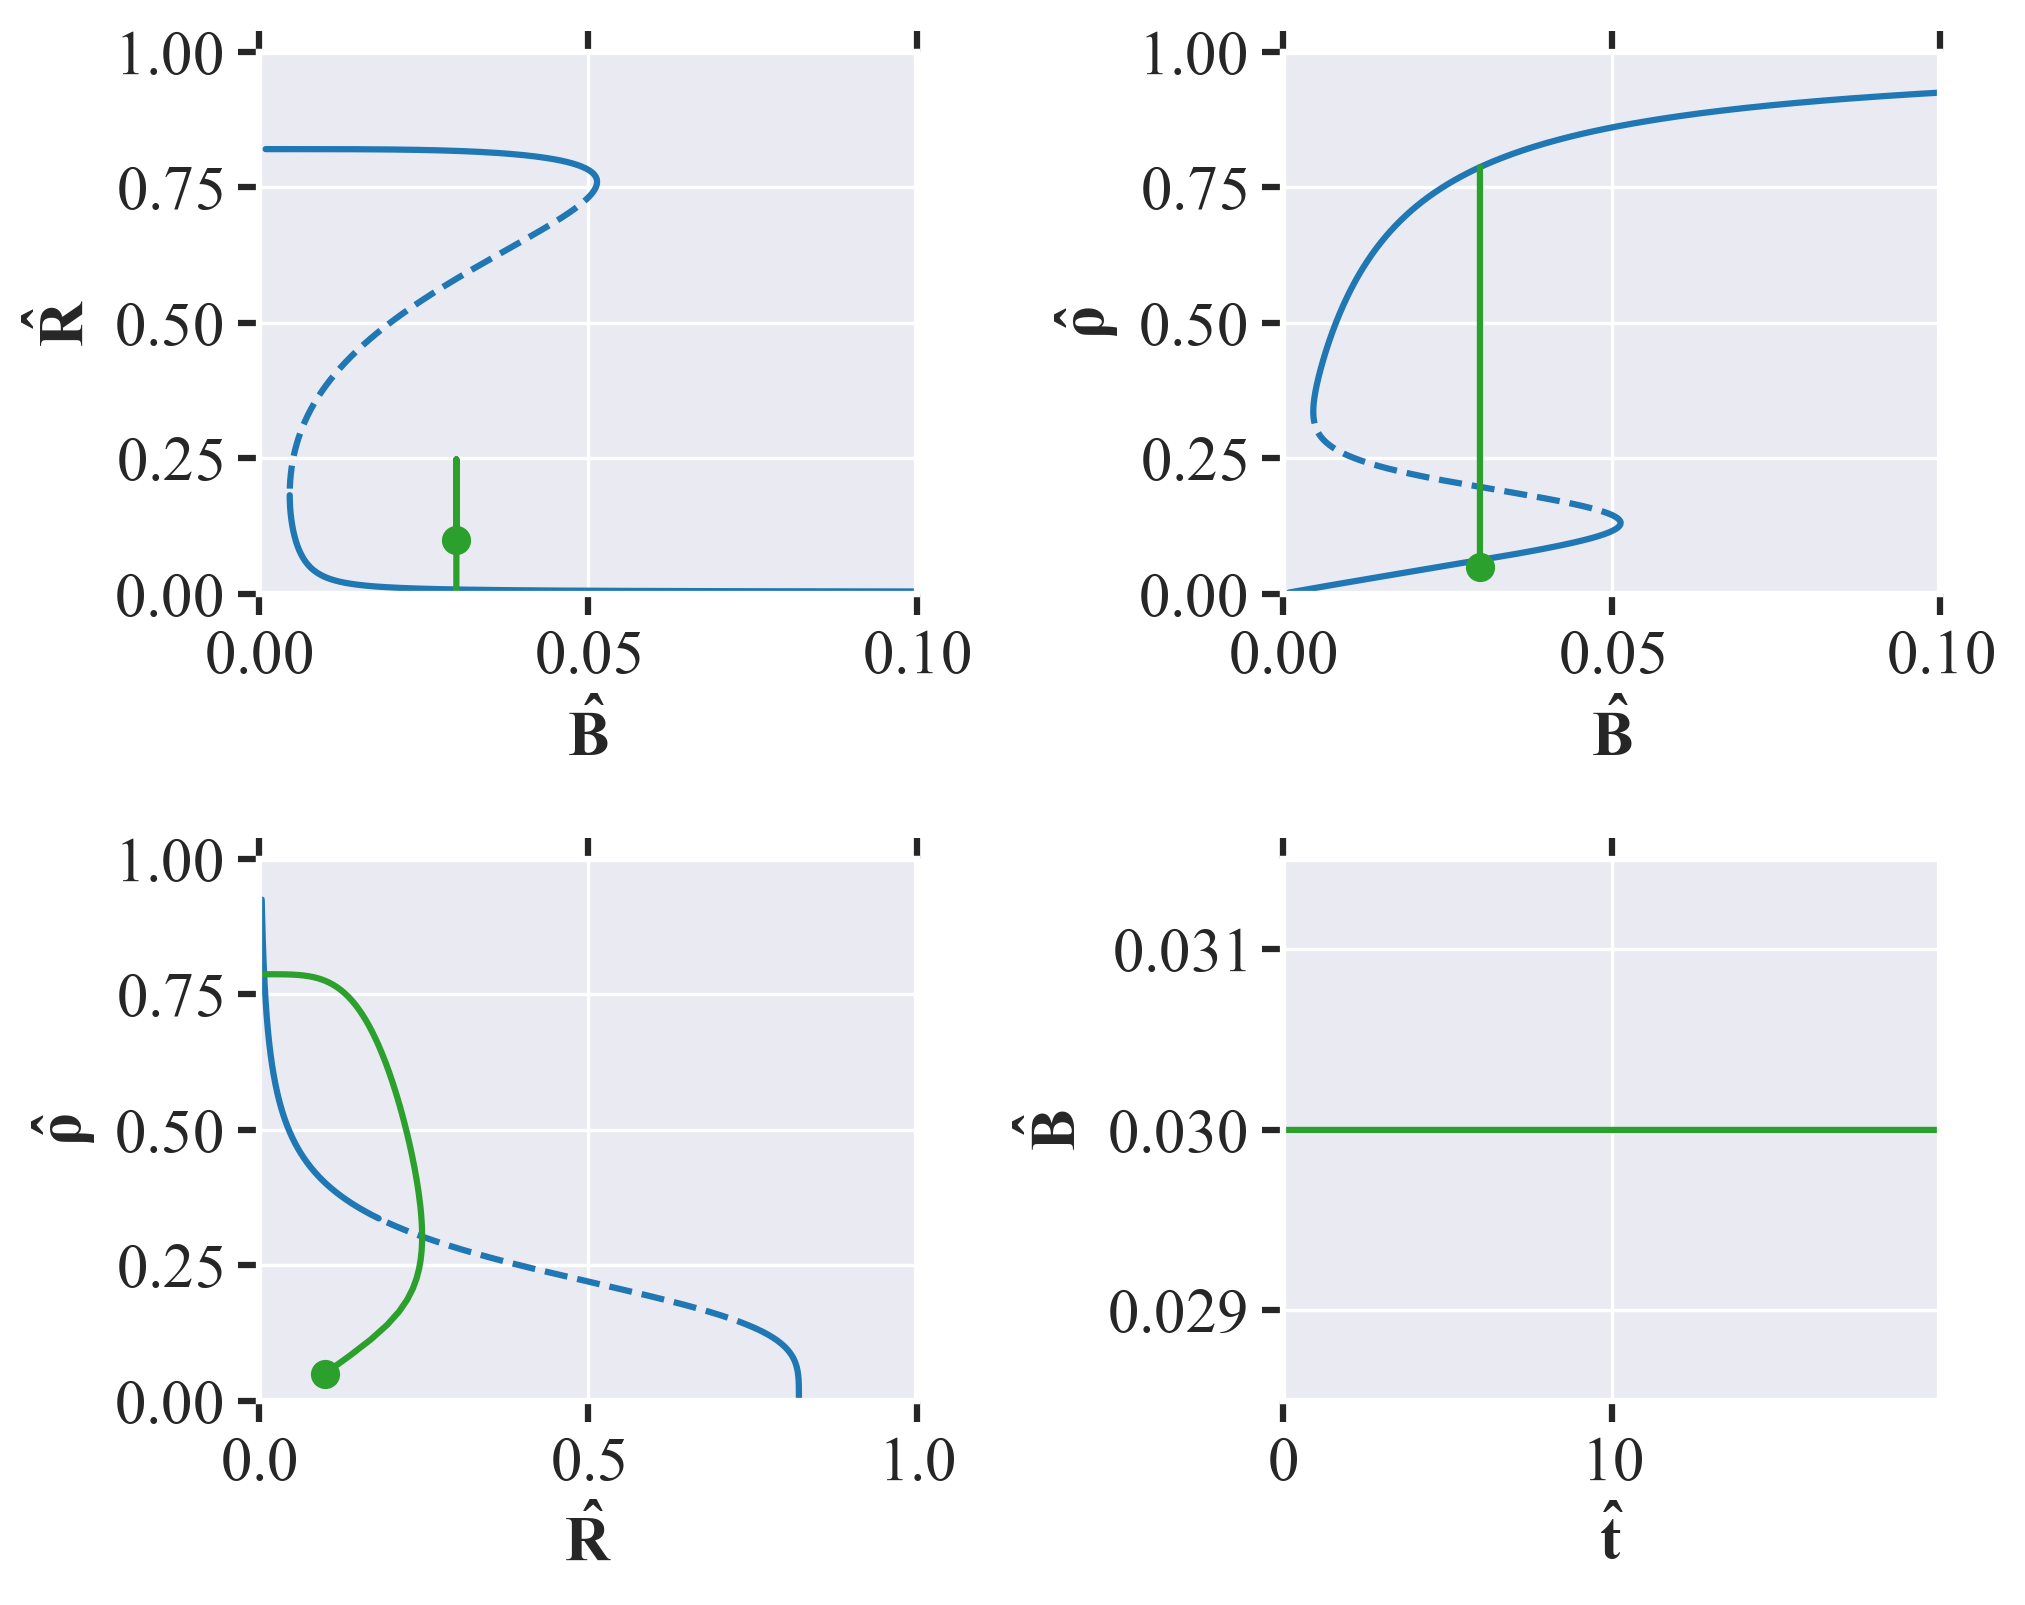
\includegraphics[width= \textwidth]{figures/cell_biology_R0=0.3_rho0=0.16_deltaR=1_n=4_Bmax=0.04_eps=0.0.png}
    \caption{Figure of the continuation of \textbf{top left:} $(\hat{R}, \hat{B})$ and \textbf{top right:}, $(\hat{\rho}, \hat{B})$, \textbf{bottom left:} phase space $(\hat{\rho}, \hat{R})$ and 
    \textbf{bottom right:} $\hat{B}$ against time (time horizon of 20 seconds with a time step of 0.01). Dots (orange) indicate turning points.}
    \label{fig:cell_biology_ex1}
\end{figure}

The system is at this stage effectively autonomous, since $\hat{B}(\hat{t}) \equiv \hat{B}_c$ is taken to be constant. Continuation is subsequently done with respect to the parameter $\hat{B}$. We observe two turning point bifurcations at:
\begin{enumerate}
    \item $\hat{B} \approx 0.051, \hat{R}\approx0.759, \hat{\rho}\approx0.131$; 
    \item $\hat{B} \approx 0.005, \hat{R}\approx0.182, \hat{\rho}\approx0.337$.
\end{enumerate}

Using the graph to get initial guesses for our Newton root finding method, we find there exist three equilibrium:
\begin{align*}
    E_0=(\hat{R_a}, \hat{\rho_a}) \approx (0.58,0.20) \leftarrow ||E_0|| \approx 0.61, \\
    E_1=(\hat{R_a}, \hat{\rho_a}) \approx (0.01,0.79) \leftarrow ||E_1|| \approx 0.79, \\
    E_2=(\hat{R_a}, \hat{\rho_a}) \approx (0.82,0.06) \leftarrow ||E_2|| \approx 0.82.
\end{align*}
$E_0$ is unstable, while $E_1$ and $E_2$ are stable. Moreover, looking at the trajectory in the phase space $(\hat{\rho}, \hat{R})$, we see that the system converges to $E_1$. 
Therefore, $E_1$ is the attractor in this case.

In figure \ref{fig:cell_biology_domains_of_attraction} the domains of attraction of $E_i, \ i = 1,2,3$ are shown.
\begin{figure}[H]
    \centering
    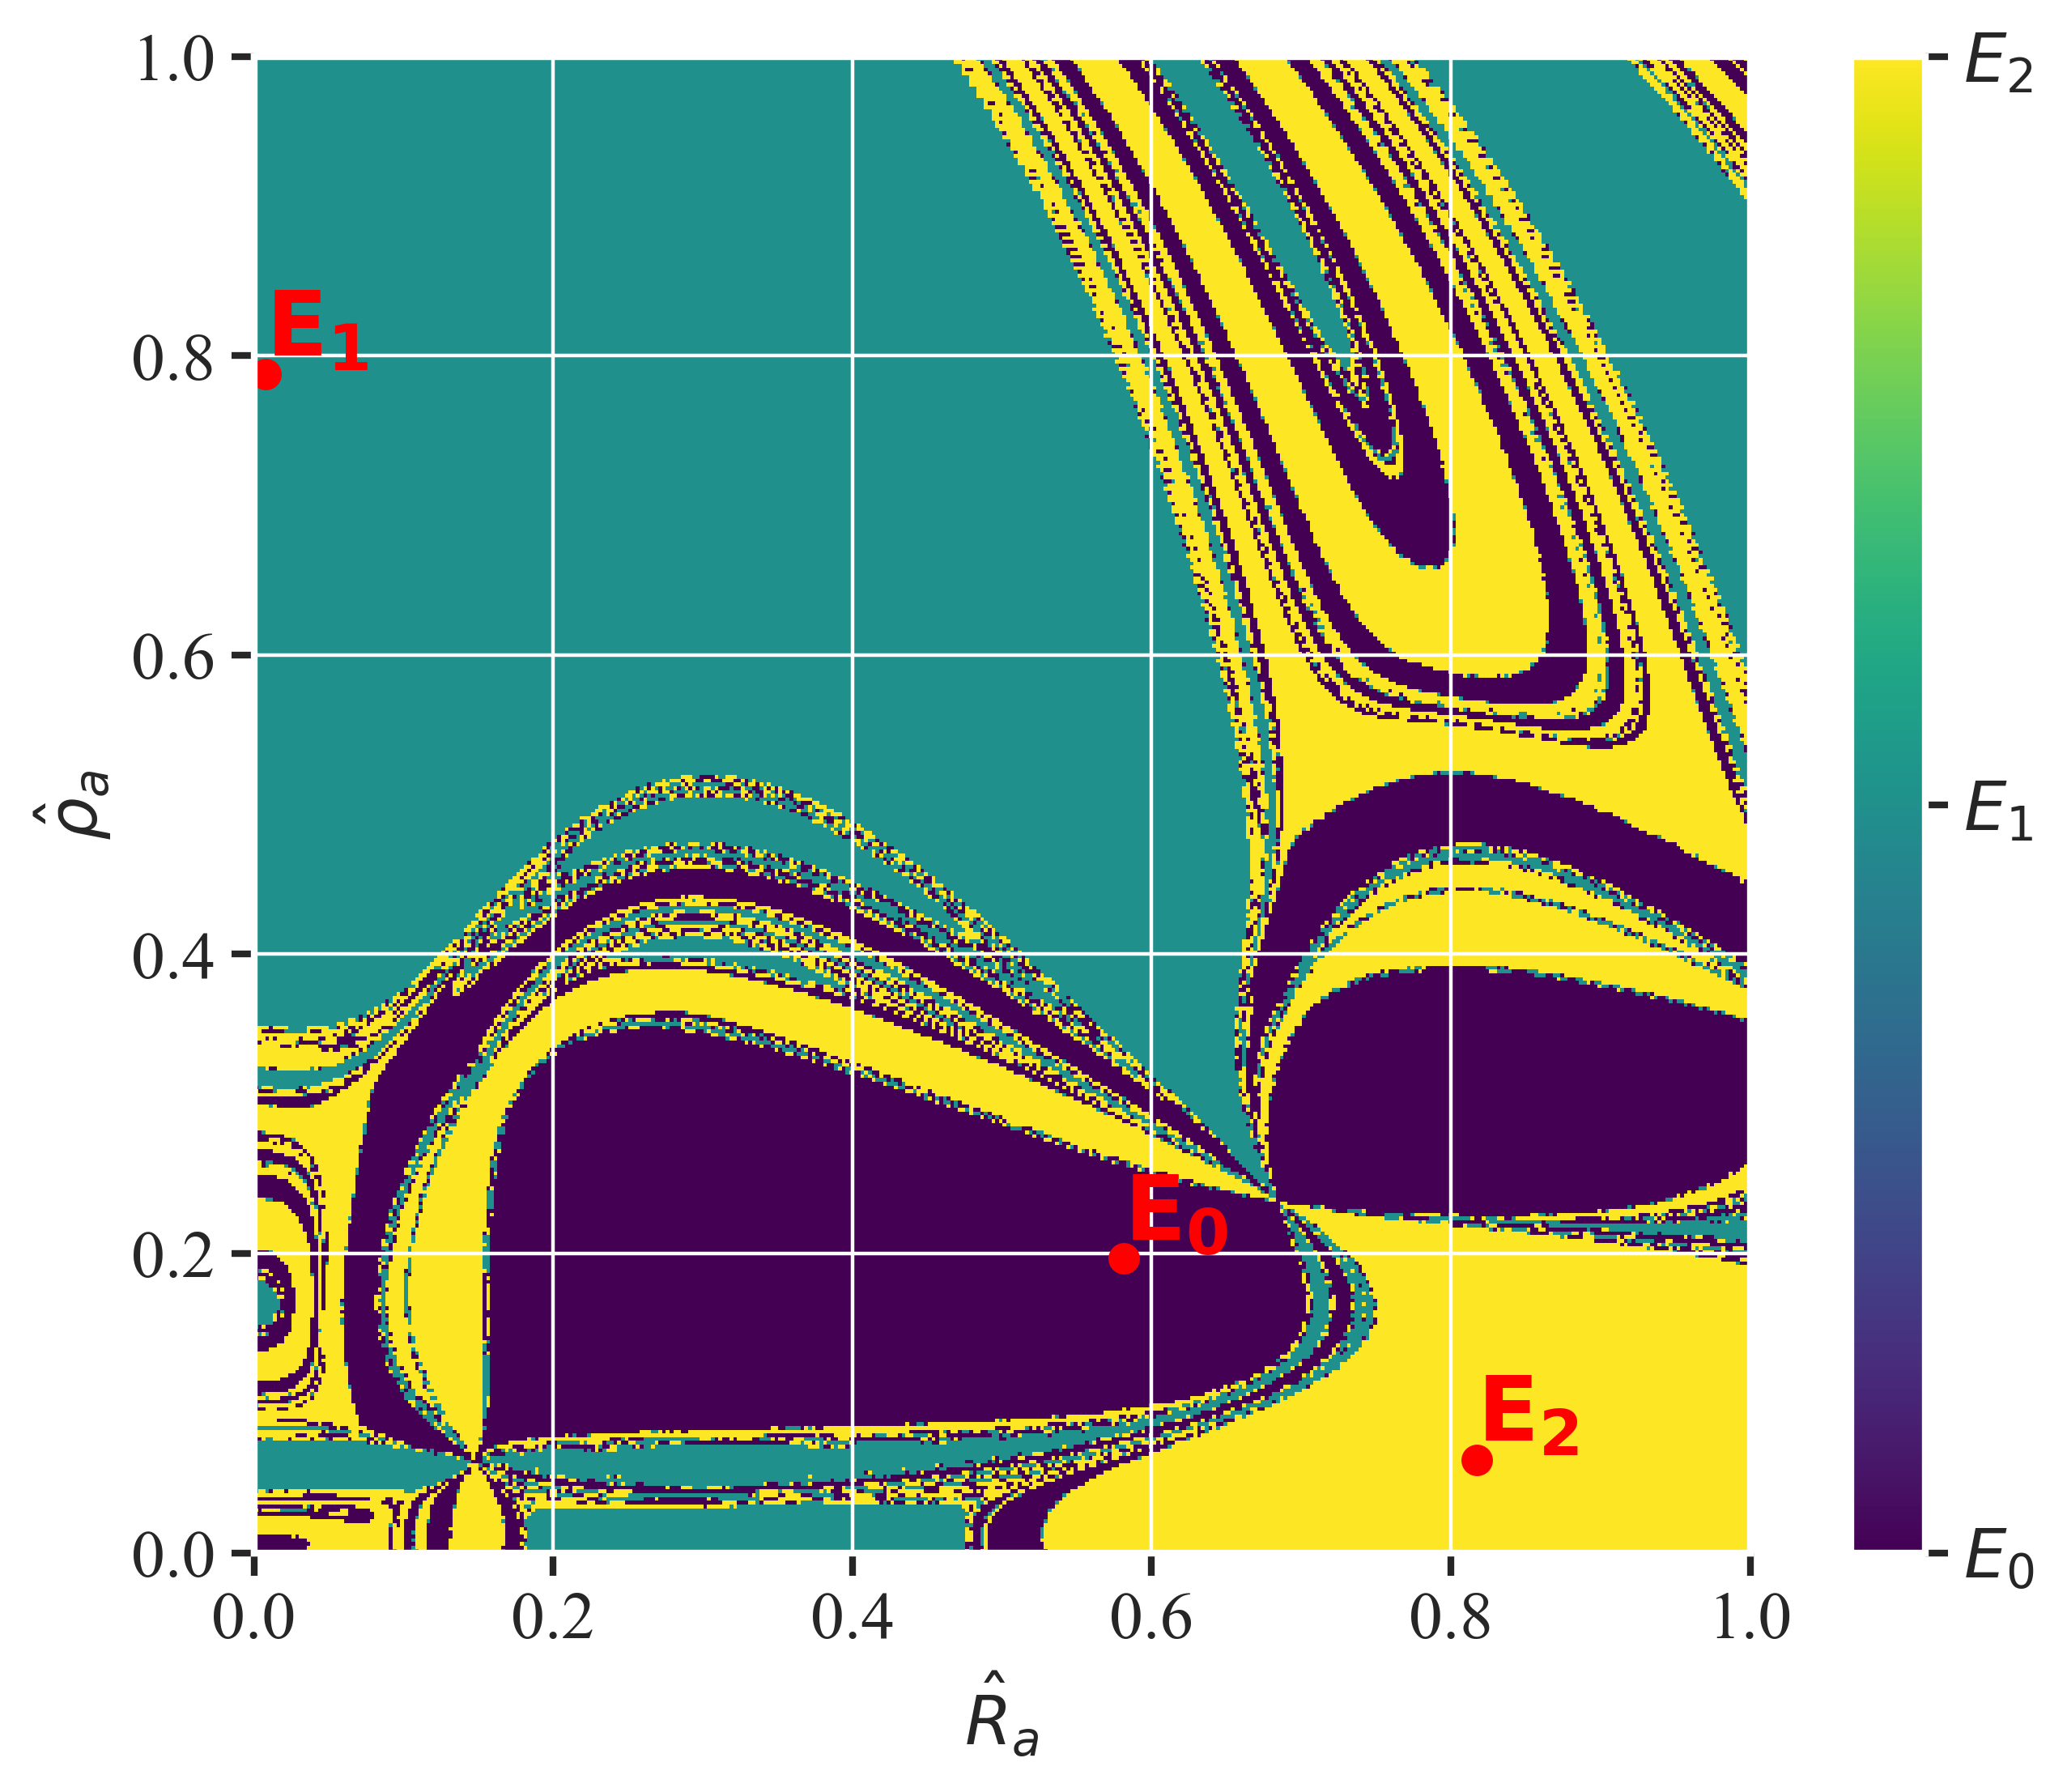
\includegraphics[width= \textwidth]{figures/cb_domains_of_attraction.png}
    \caption{Domains of attraction of $E_i, \ i = 1,2,3$}
    \label{fig:cell_biology_domains_of_attraction}
\end{figure}

\subsection{Non-autonomous system}
We now introduce a `small' linear time-dependent perturbation to $\hat{B}$. That is, the perturbed system is now given by
\begin{align*}
    \hat{R}'_a &= \frac{\hat{A} \left(1 - \hat{R}_{a}\right)}{\hat{\rho}_a^{n} + \rho_{0}^{n}}  - \hat{\delta}_{R} \hat{R}_{a}\\
    \hat{\rho}'_a &= \frac{\hat{B} \left(1 - \hat{\rho}_a\right)}{\hat{R}_0^{n} + \hat{R}_{a}^{n}} - \hat{\rho}_a\\
    \hat{B}' &= \epsilon,
\end{align*}
where $\epsilon$ is small or big with respect to the system dynamics (reciprocal of the linearized system's eigenvalues). 

Figures \ref{fig:cell_biology_ex3_small} and \ref{fig:cell_biology_ex3_big} show the continuation of the system with $\epsilon = 0.001$ and $\epsilon = 0.01$ respectively.
\begin{figure}[H]
    \centering
    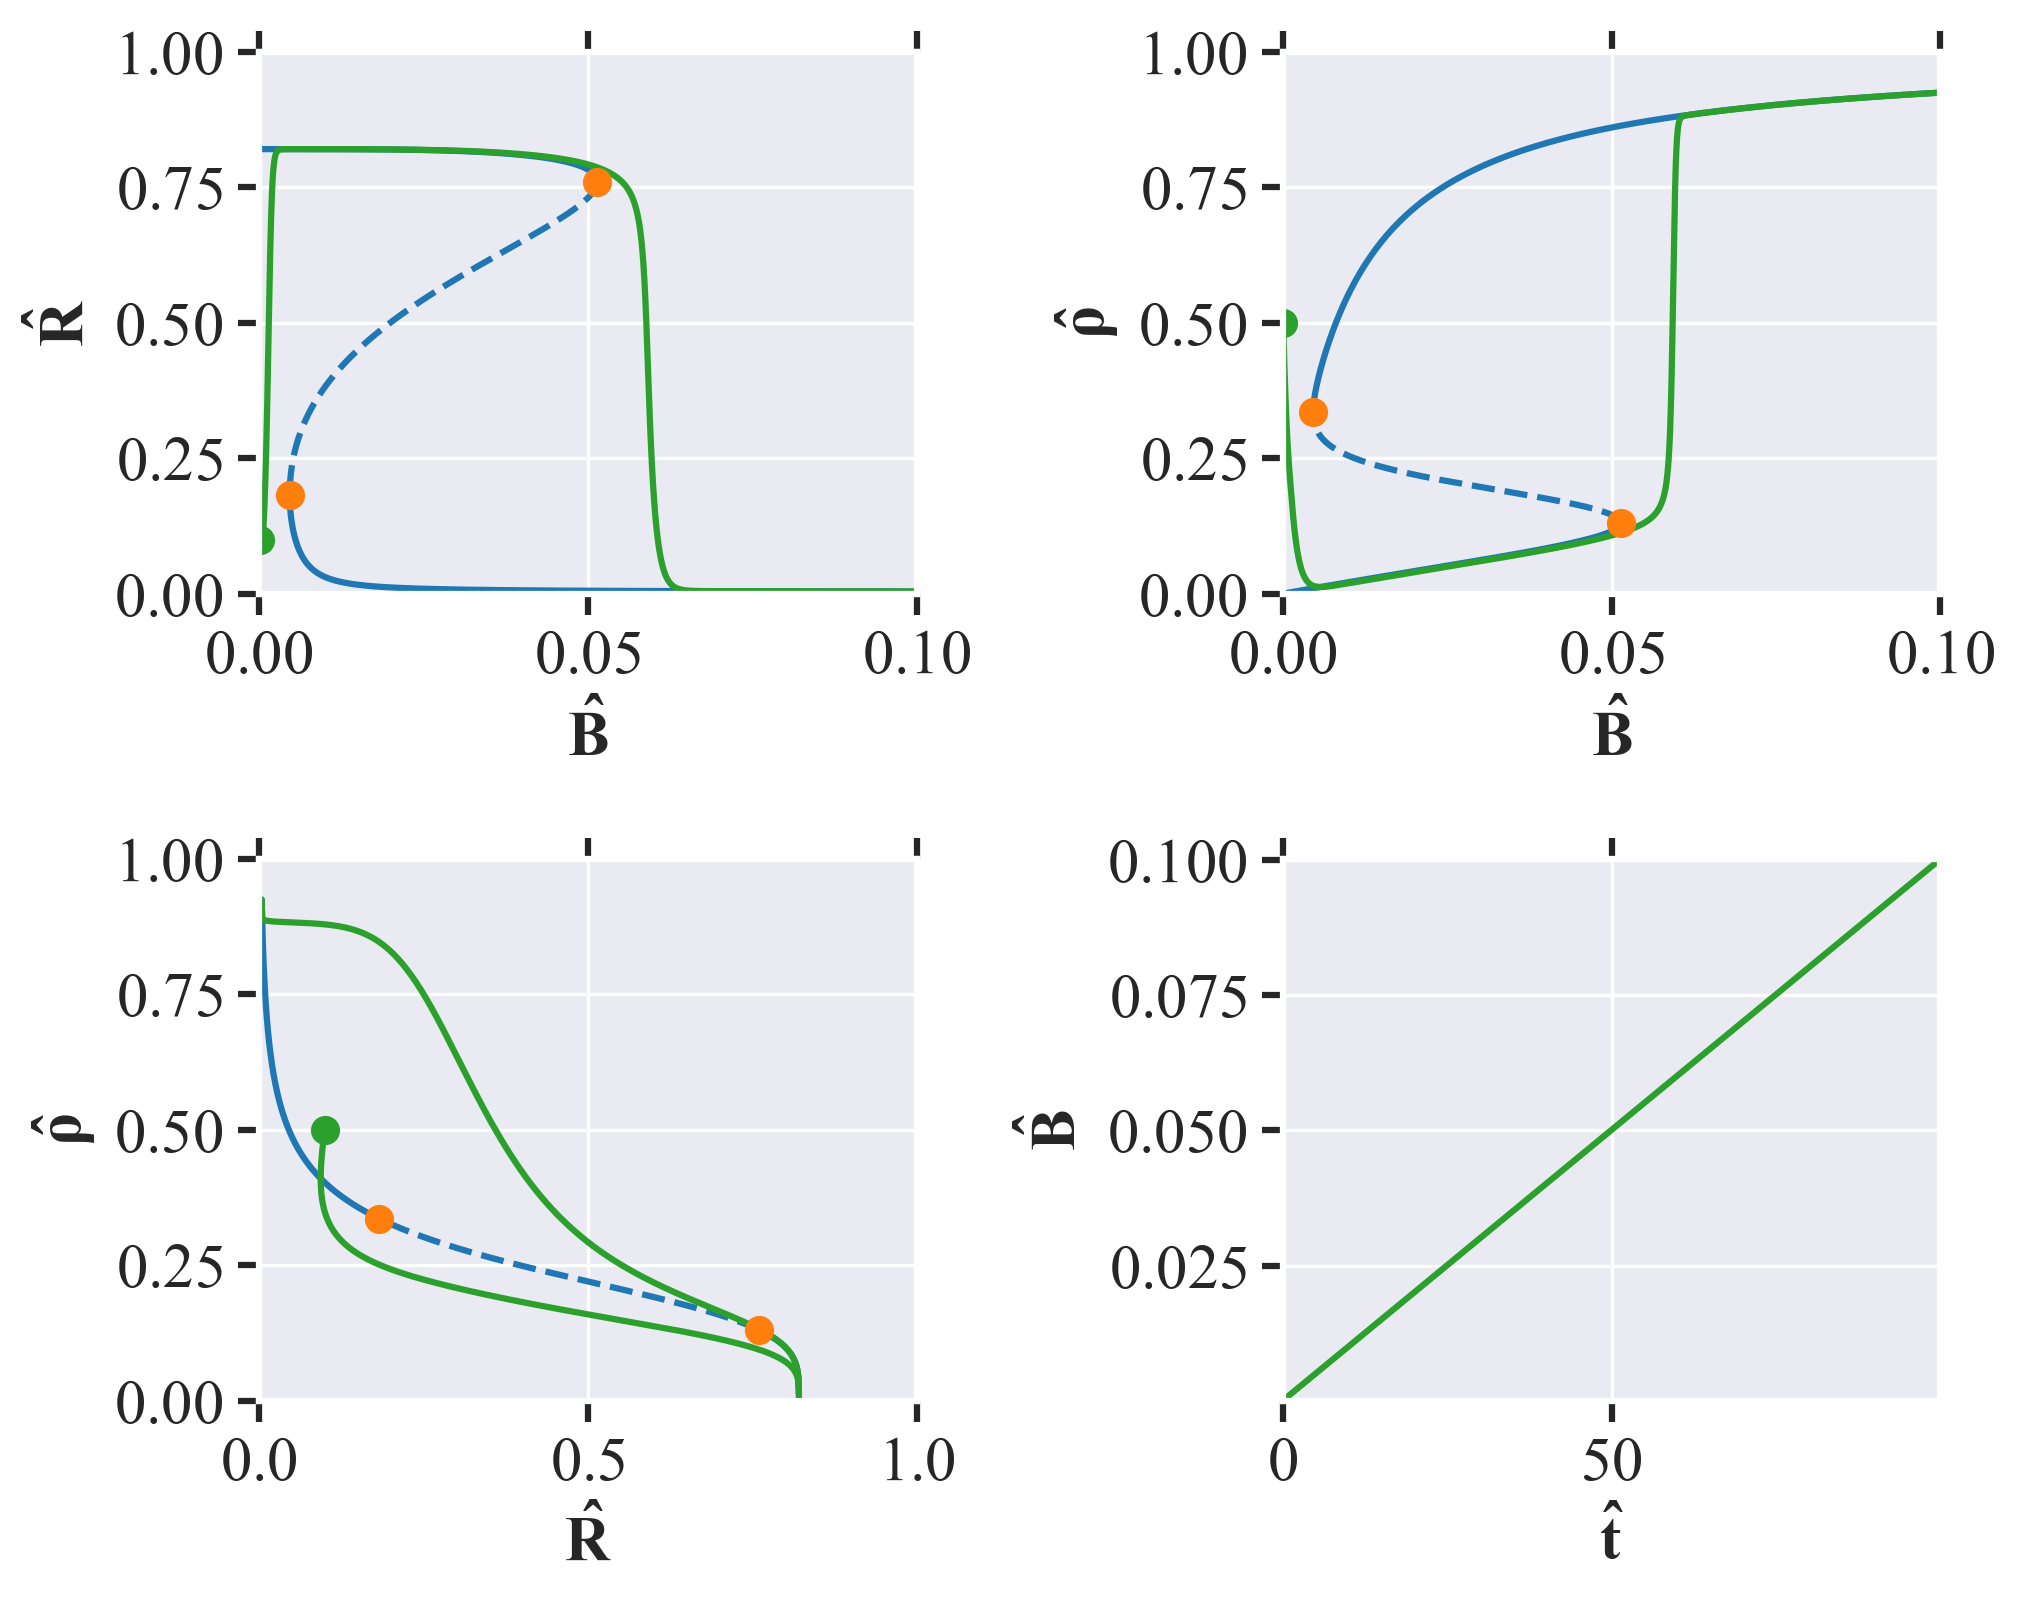
\includegraphics[width= \textwidth]{figures/cell_biology_R(0)=0.1_rho(0)=0.5_B(0)_0.0001_eps=0.001_Bmax=0.04.png}
    \caption{}
    \label{fig:cell_biology_ex3_small}
\end{figure}

\begin{figure}[H]
    \centering
    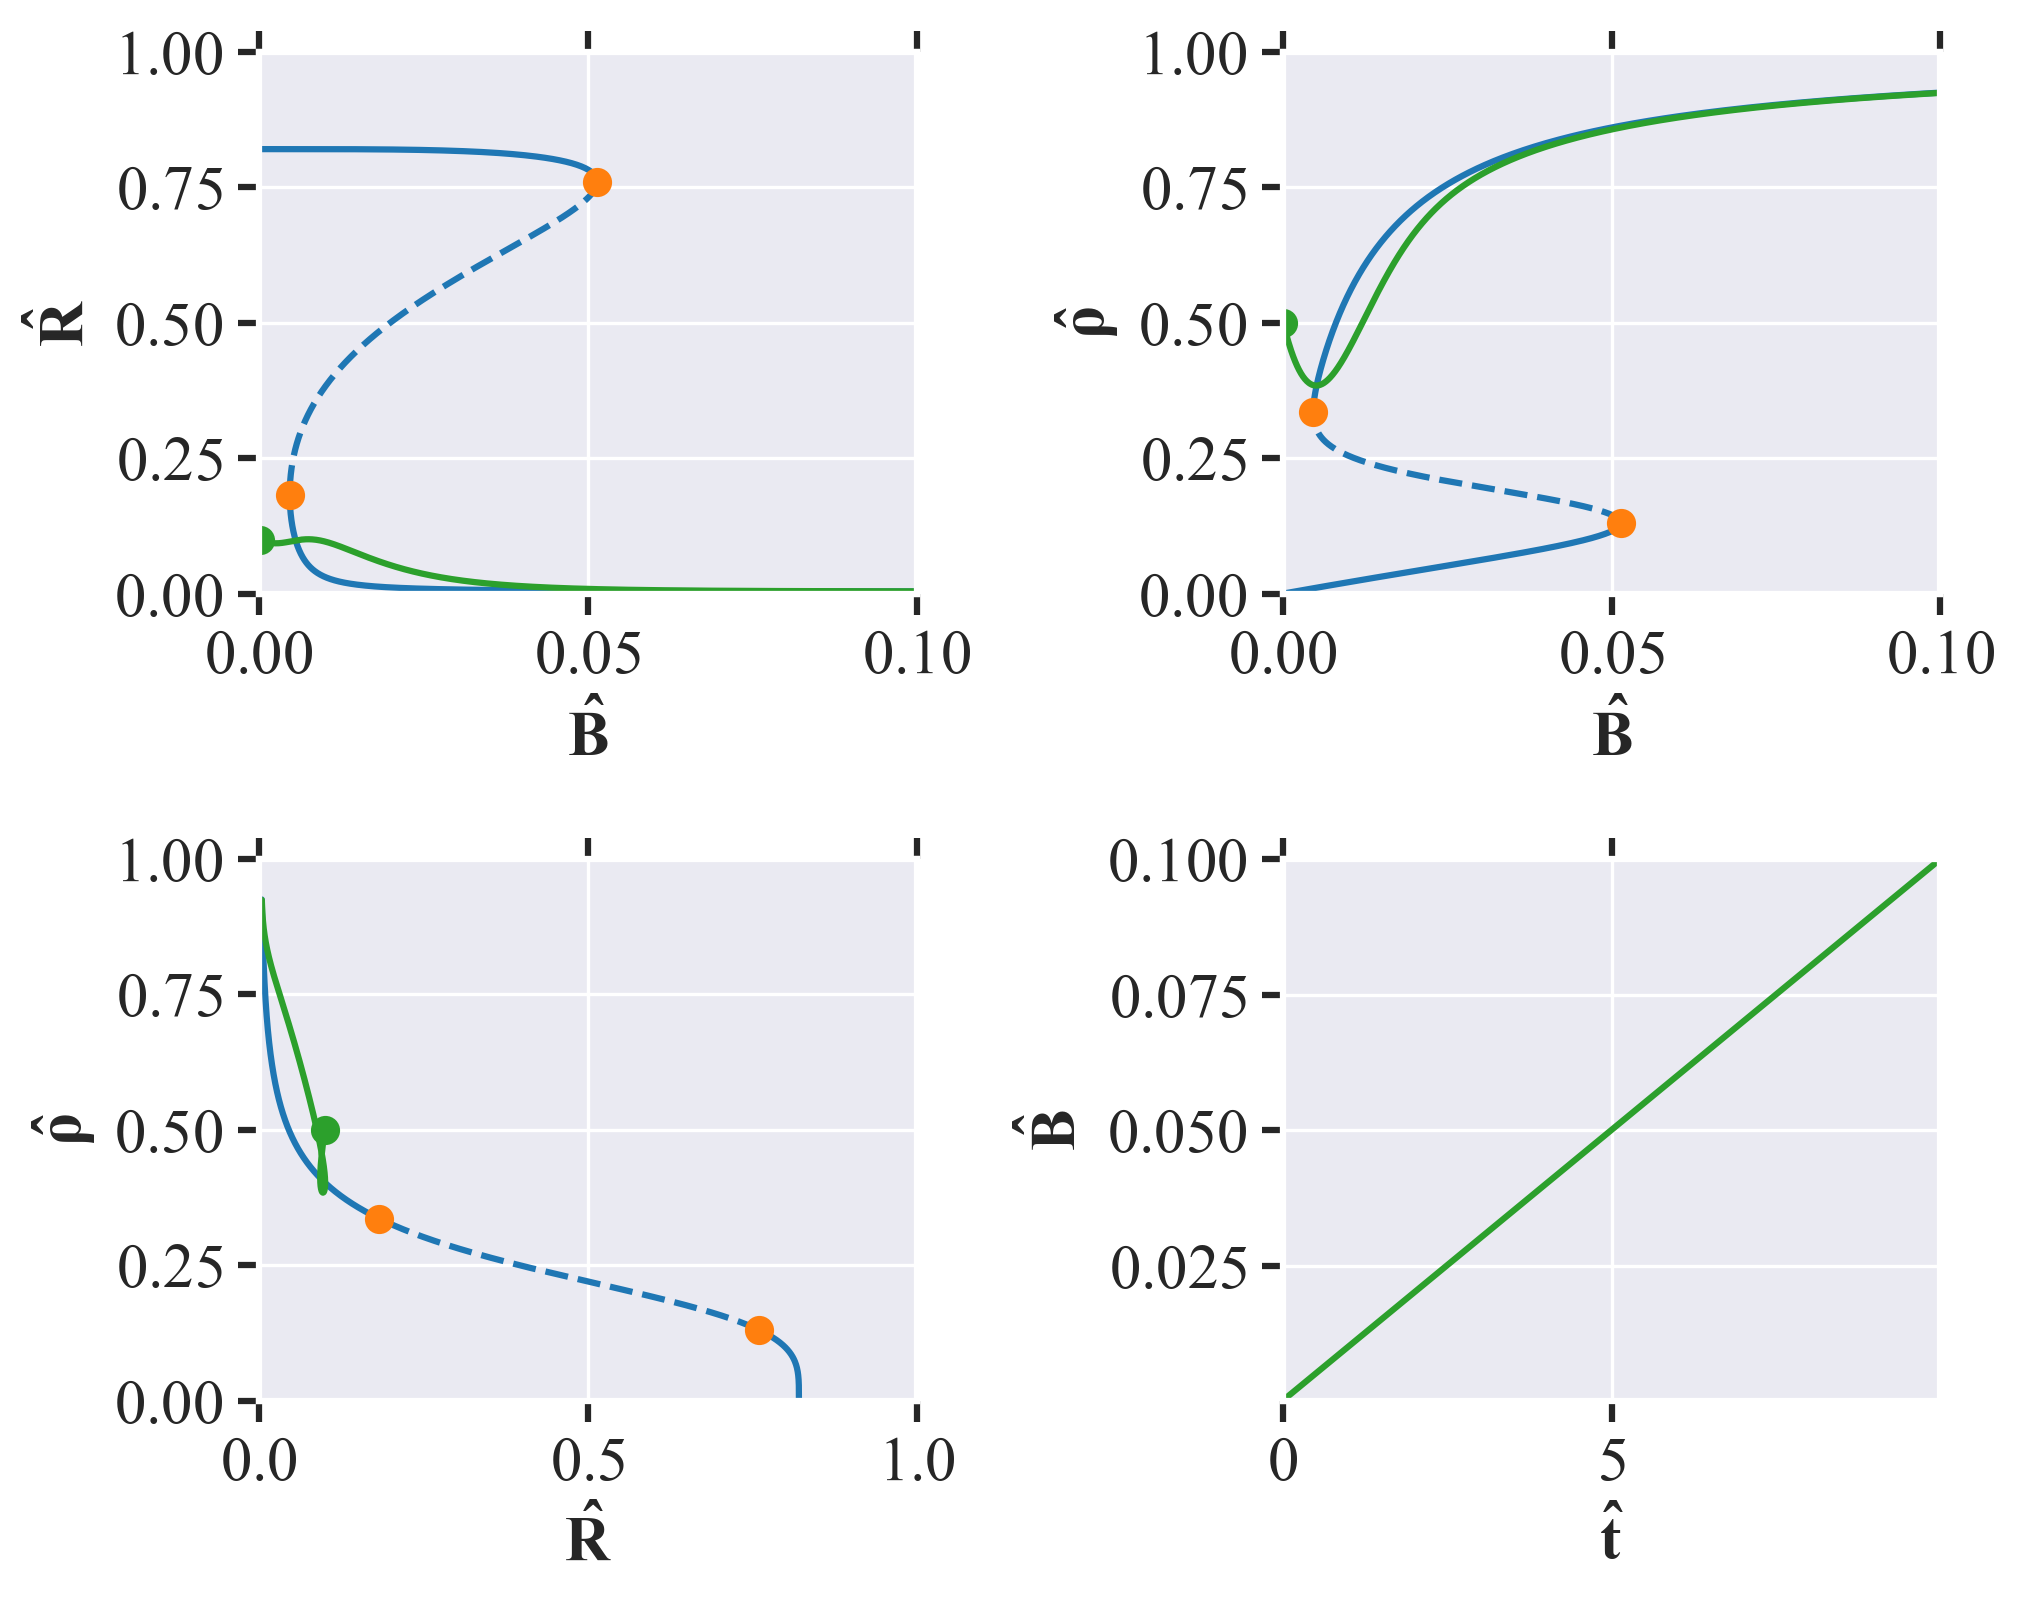
\includegraphics[width= \textwidth]{figures/cell_biology_R(0)=0.1_rho(0)=0.5_B(0)_0.0001_eps=0.01_Bmax=0.04.png}
    \caption{...}
    \label{fig:cell_biology_ex3_big}
\end{figure}

Next, we look for critical slowing down near the bifurcations of the system. The results for $\epsilon = 0.001$ and $\epsilon = 0.01$ are shown in figures \ref{fig:cell_biology_critical_slowing_down_small} and \ref{fig:cell_biology_critical_slowing_down_big} respectively.
\begin{figure}[H]
    \centering
    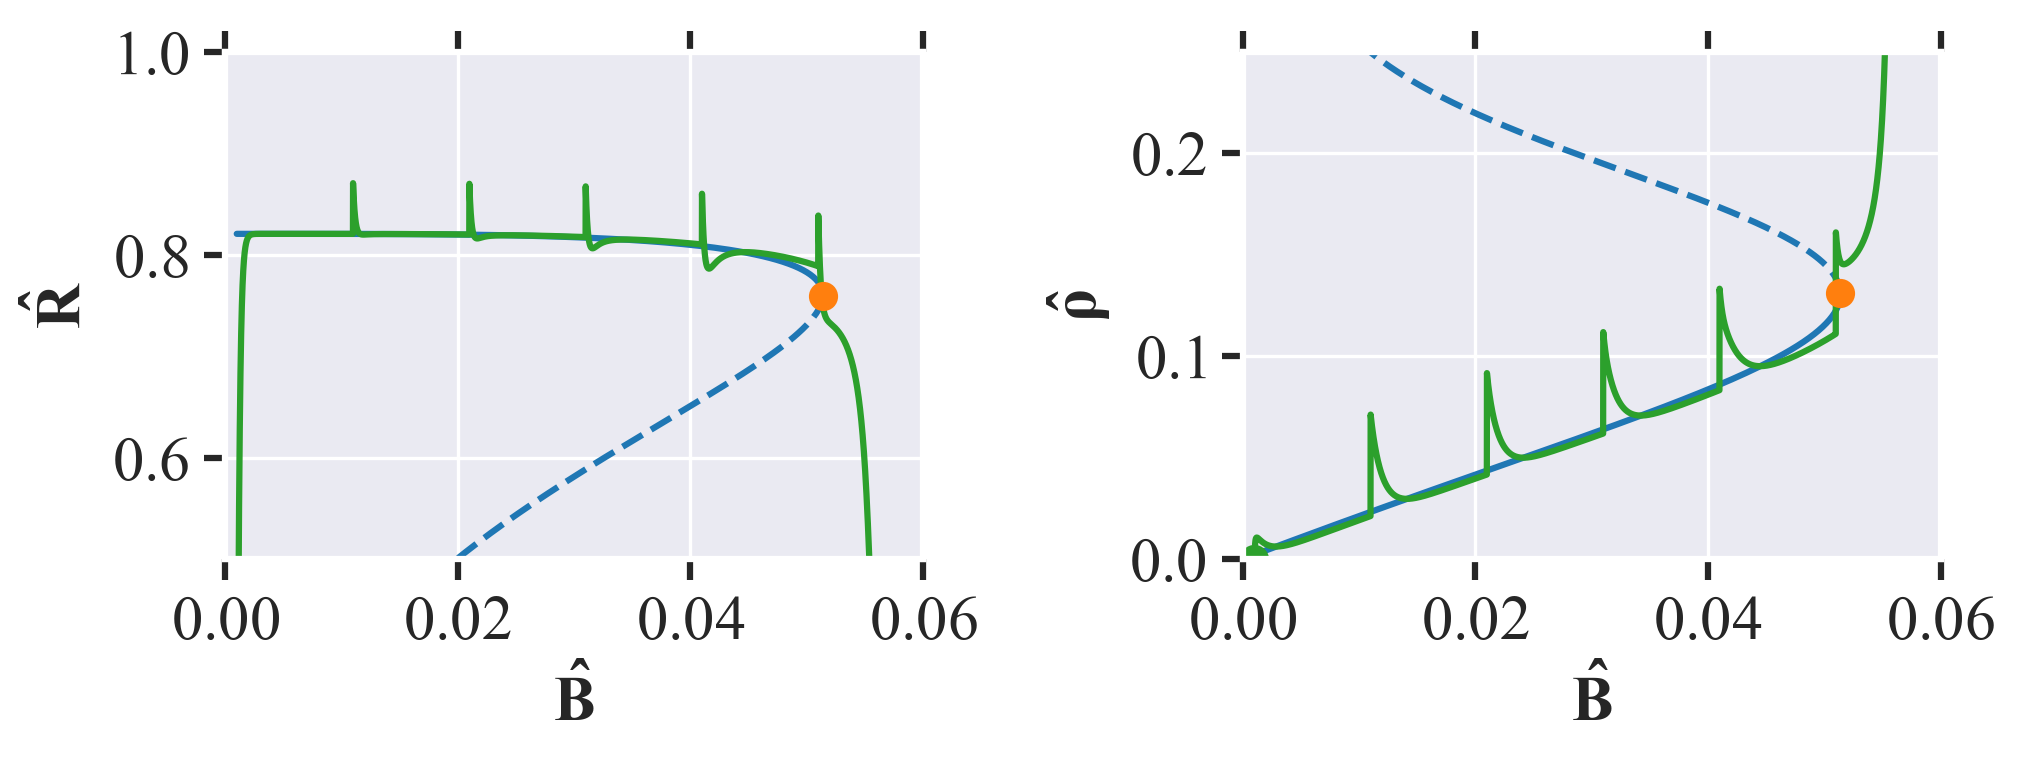
\includegraphics[width= \textwidth]{figures/cb_critslow_R(0)=0.0_rho(0)=0.0_B(0)_0.001_eps=0.001_Bmax=0.04.png}
    \caption{...}
    \label{fig:cell_biology_critical_slowing_down_small}
\end{figure}

\begin{figure}[H]
    \centering
    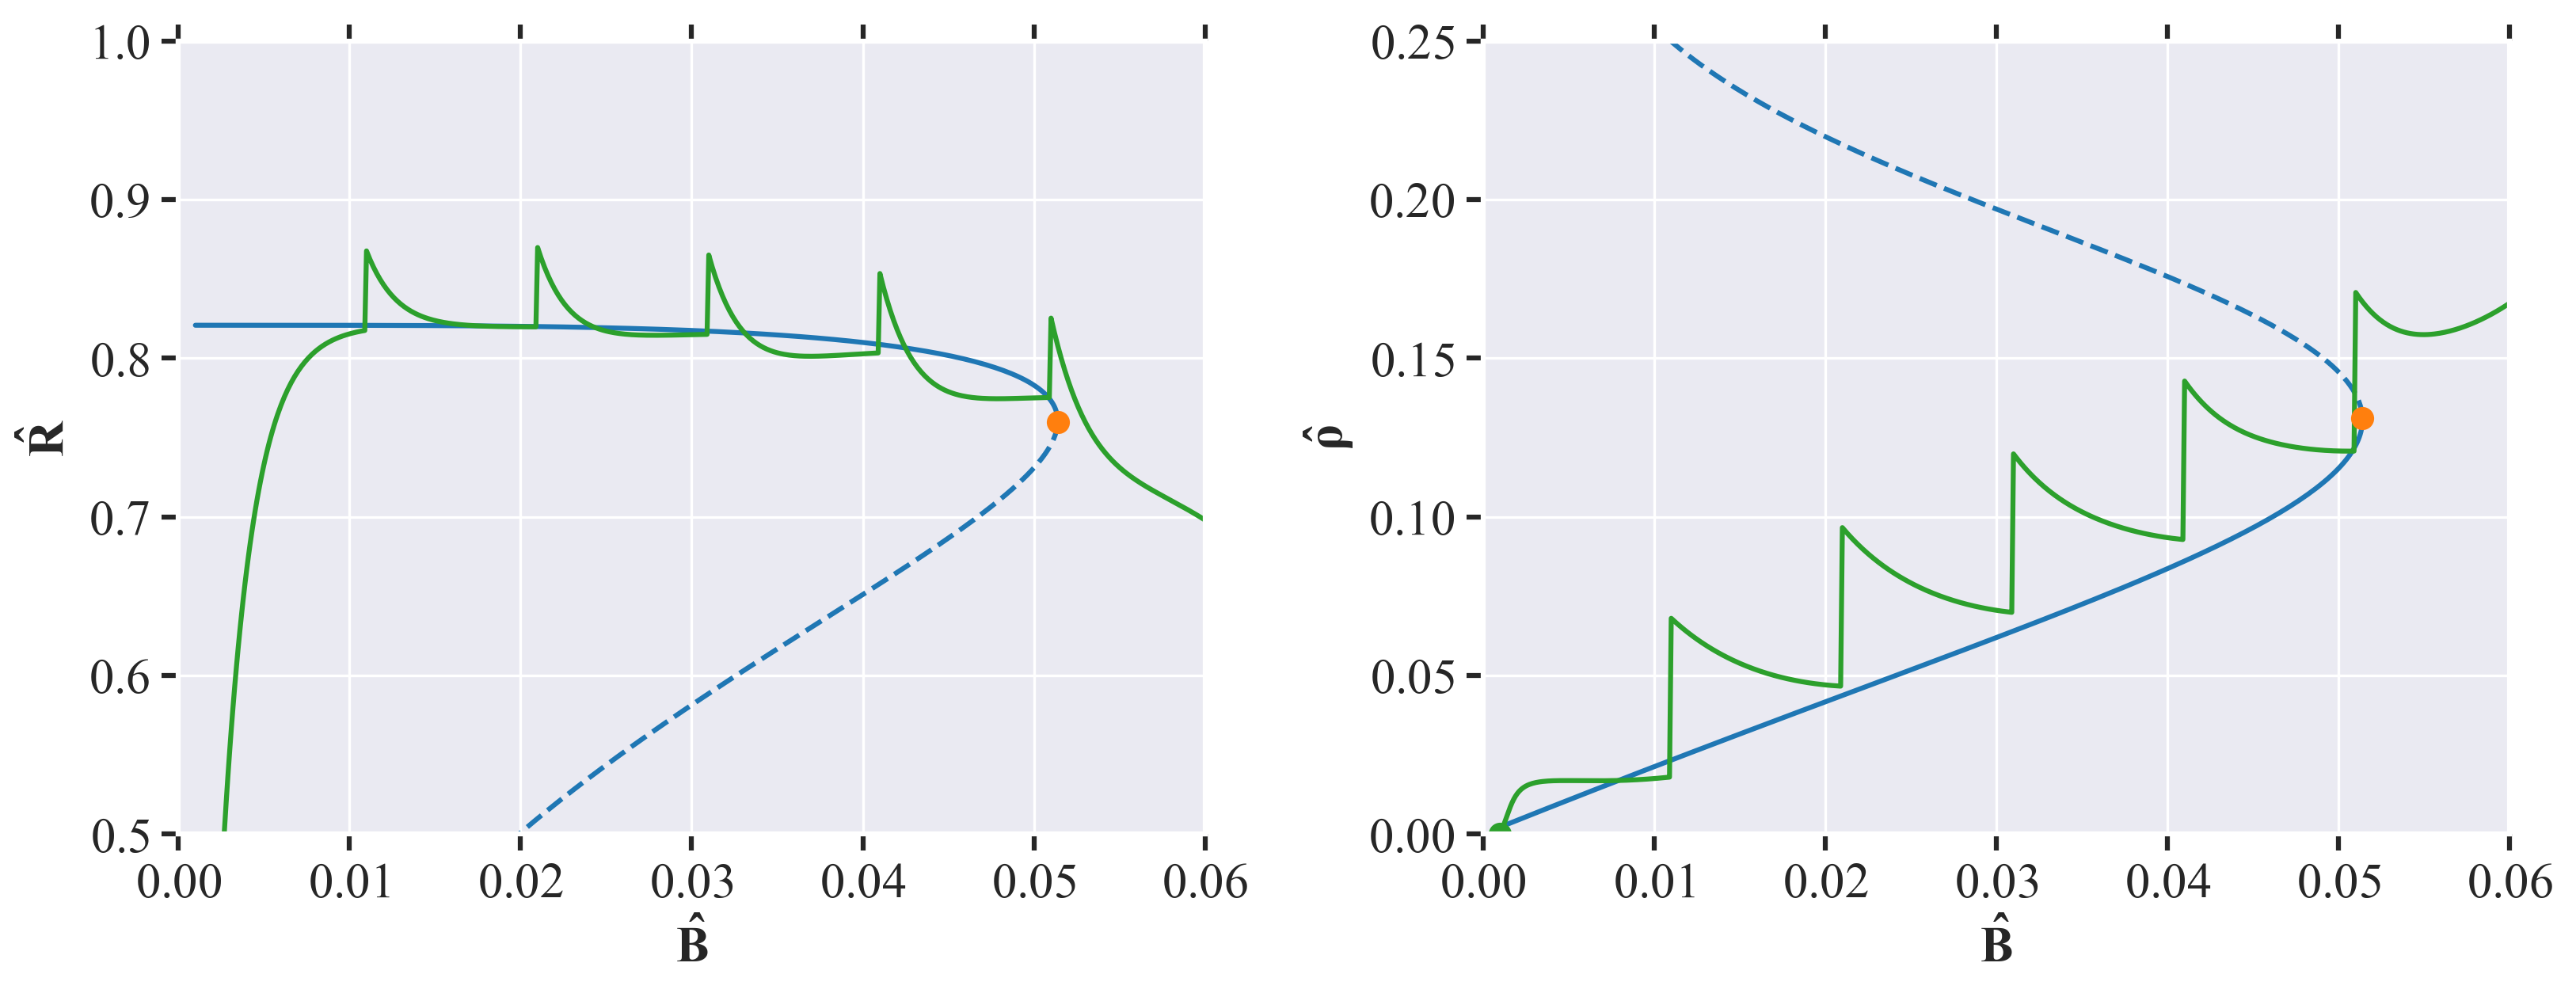
\includegraphics[width= \textwidth]{figures/cb_critslow_R(0)=0.0_rho(0)=0.0_B(0)_0.001_eps=0.01_Bmax=0.04.png}
    \caption{..}
    \label{fig:cell_biology_critical_slowing_down_big}
\end{figure}

\subsection{Conclusion}
\todo{Conclusion to the assignment}